% Generated by `seq-lang draw --format tikz`. Do not edit by hand.
% Requires \usepackage{tikz}.
\definecolor{seqink}{HTML}{1D2021}
\definecolor{seqdim}{HTML}{6B7280}
\definecolor{seqline}{HTML}{4B5563}
\definecolor{seqfill}{HTML}{EEF2F5}
\definecolor{seqtint}{HTML}{D8E6E4}
\definecolor{seqcache}{HTML}{E6E2DA}
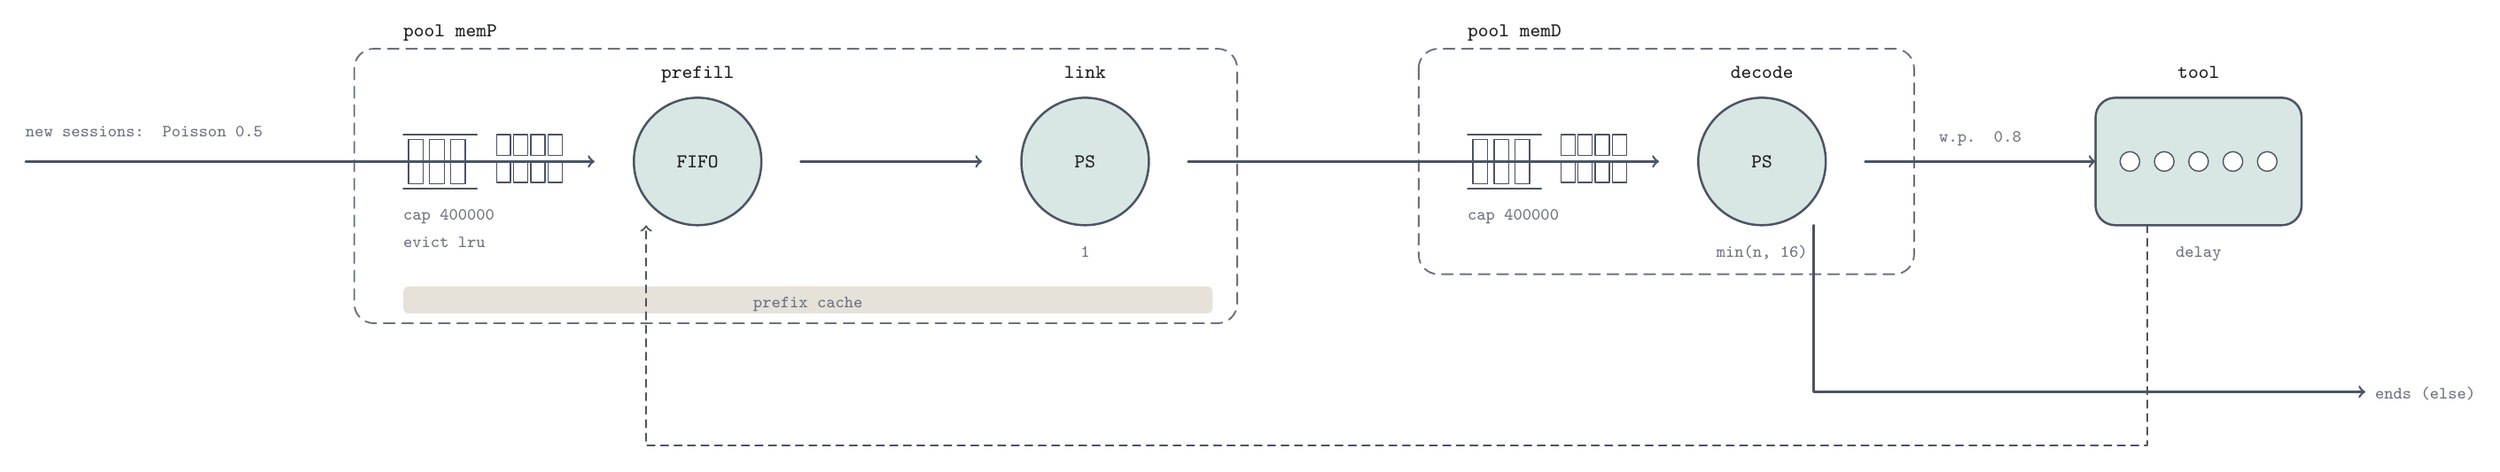
\begin{tikzpicture}[x=1pt, y=-1pt, line cap=round, line join=round,
  every node/.style={inner sep=0pt, outer sep=0pt, text=seqink},
  seqsolid/.style={draw=seqline, fill=seqfill, line width=.8pt},
  seqbody/.style={draw=seqline, fill=seqfill, line width=.8pt},
  seqadmission/.style={draw=seqline, fill=seqfill, line width=.8pt, dash pattern=on 4pt off 2.5pt},
  seqcached/.style={draw=none, fill=seqcache},
  seqfits/.style={draw=seqdim, line width=.5pt, dash pattern=on 1.5pt off 2.5pt},
  seqenclosure/.style={draw=seqdim, line width=.7pt, dash pattern=on 4.5pt off 3pt},
  seqstation/.style={draw=seqline, fill=seqtint, line width=.9pt},
  seqcell/.style={draw=seqline, fill=white, line width=.5pt},
  seqrail/.style={draw=seqline, line width=.7pt},
  seqflow/.style={draw=seqline, line width=.9pt, ->},
  seqback/.style={draw=seqline, line width=.8pt, dash pattern=on 3pt off 2.5pt, ->},
  seqrelation/.style={draw=seqdim, line width=.7pt, dash pattern=on 1.5pt off 2.5pt, ->},
  seqgrow/.style={draw=seqline, line width=.7pt, ->}]
  \draw[rounded corners=8pt, seqenclosure] (162,57) rectangle (522,169);
  \node[anchor=base west] at (182,52) {\ttfamily\footnotesize pool memP};
  \draw[seqrail] (182,92) -- (212,92);
  \draw[seqrail] (182,114) -- (212,114);
  \draw[seqcell] (184.14,94) rectangle (190.14,112);
  \draw[seqcell] (192.71,94) rectangle (198.71,112);
  \draw[seqcell] (201.29,94) rectangle (207.29,112);
  \draw[seqcell] (220,92) rectangle (225.74,100.58);
  \draw[seqcell] (227,92) rectangle (232.74,100.58);
  \draw[seqcell] (234,92) rectangle (239.74,100.58);
  \draw[seqcell] (241,92) rectangle (246.74,100.58);
  \draw[seqcell] (220,103) rectangle (225.74,111.58);
  \draw[seqcell] (227,103) rectangle (232.74,111.58);
  \draw[seqcell] (234,103) rectangle (239.74,111.58);
  \draw[seqcell] (241,103) rectangle (246.74,111.58);
  \node[text=seqdim, anchor=base west] at (182,127) {\ttfamily\scriptsize cap 400000};
  \node[text=seqdim, anchor=base west] at (182,138) {\ttfamily\scriptsize evict lru};
  \draw[rounded corners=2pt, seqcached] (182,154) rectangle (512,165);
  \node[text=seqdim, anchor=base] at (347,162.5) {\ttfamily\scriptsize prefix cache};
  \draw[rounded corners=8pt, seqenclosure] (596,57) rectangle (798,149);
  \node[anchor=base west] at (616,52) {\ttfamily\footnotesize pool memD};
  \draw[seqrail] (616,92) -- (646,92);
  \draw[seqrail] (616,114) -- (646,114);
  \draw[seqcell] (618.14,94) rectangle (624.14,112);
  \draw[seqcell] (626.71,94) rectangle (632.71,112);
  \draw[seqcell] (635.29,94) rectangle (641.29,112);
  \draw[seqcell] (654,92) rectangle (659.74,100.58);
  \draw[seqcell] (661,92) rectangle (666.74,100.58);
  \draw[seqcell] (668,92) rectangle (673.74,100.58);
  \draw[seqcell] (675,92) rectangle (680.74,100.58);
  \draw[seqcell] (654,103) rectangle (659.74,111.58);
  \draw[seqcell] (661,103) rectangle (666.74,111.58);
  \draw[seqcell] (668,103) rectangle (673.74,111.58);
  \draw[seqcell] (675,103) rectangle (680.74,111.58);
  \node[text=seqdim, anchor=base west] at (616,127) {\ttfamily\scriptsize cap 400000};
  \draw[seqstation] (302,103) circle (26pt);
  \node[anchor=center] at (302,103) {\ttfamily\footnotesize FIFO};
  \node[anchor=base] at (302,69) {\ttfamily\footnotesize prefill};
  \draw[seqstation] (460,103) circle (26pt);
  \node[anchor=center] at (460,103) {\ttfamily\footnotesize PS};
  \node[anchor=base] at (460,69) {\ttfamily\footnotesize link};
  \node[text=seqdim, anchor=base] at (460,142) {\ttfamily\scriptsize 1};
  \draw[seqstation] (736,103) circle (26pt);
  \node[anchor=center] at (736,103) {\ttfamily\footnotesize PS};
  \node[anchor=base] at (736,69) {\ttfamily\footnotesize decode};
  \node[text=seqdim, anchor=base] at (736,142) {\ttfamily\scriptsize min(n, 16)};
  \draw[seqstation, rounded corners=8pt] (872,77) rectangle (956,129);
  \draw[seqcell] (886,103) circle (4pt);
  \draw[seqcell] (900,103) circle (4pt);
  \draw[seqcell] (914,103) circle (4pt);
  \draw[seqcell] (928,103) circle (4pt);
  \draw[seqcell] (942,103) circle (4pt);
  \node[anchor=base] at (914,69) {\ttfamily\footnotesize tool};
  \node[text=seqdim, anchor=base] at (914,142) {\ttfamily\scriptsize delay};
  \draw[seqflow] (28,103) -- (260,103);
  \node[text=seqdim, anchor=base west] at (28,93) {\ttfamily\scriptsize new sessions: Poisson 0.5};
  \draw[seqflow] (344,103) -- (418,103);
  \draw[seqflow] (502,103) -- (694,103);
  \draw[seqflow] (778,103) -- (872,103);
  \node[text=seqdim, anchor=base] at (825,95) {\ttfamily\scriptsize w.p. 0.8};
  \draw[seqflow] (757,129) -- (757,197) -- (982,197);
  \node[text=seqdim, anchor=base west] at (986,200) {\ttfamily\scriptsize ends (else)};
  \draw[seqback] (893,129) -- (893,219) -- (281,219) -- (281,129);
\end{tikzpicture}
